%%%%%%%%%%%%%%%%%%%%%%%%%%%%%%%%%%%%%%%%%
% Simple Sectioned Essay Template
% LaTeX Template
%
% This template has been downloaded from:
% http://www.latextemplates.com
%
% Note:
% The \lipsum[#] commands throughout this template generate dummy text
% to fill the template out. These commands should all be removed when 
% writing essay content.
%
%%%%%%%%%%%%%%%%%%%%%%%%%%%%%%%%%%%%%%%%%

%----------------------------------------------------------------------------------------
%	PACKAGES AND OTHER DOCUMENT CONFIGURATIONS
%----------------------------------------------------------------------------------------

\documentclass[12pt]{article} % Default font size is 12pt, it can be changed here

\usepackage{geometry} % Required to change the page size to A4
\geometry{a4paper} % Set the page size to be A4 as opposed to the default US Letter

\usepackage{graphicx} % Required for including pictures

\usepackage{fullpage}

\usepackage{listings}

\usepackage{amsmath}

\usepackage{float} % Allows putting an [H] in \begin{figure} to specify the exact location of the figure
\usepackage{wrapfig} % Allows in-line images such as the example fish picture
\usepackage{pdfpages}

\usepackage{subfigure}

\linespread{1.2} % Line spacing

%\setlength\parindent{0pt} % Uncomment to remove all indentation from paragraphs

\graphicspath{{Pictures/}} % Specifies the directory where pictures are stored

\usepackage[numbered, framed]{matlab-prettifier}

\title{Advanced Statistical Machine Learning \\ Assignment \#1}
\author{
	Robert Webb, (rjw14), \\
	Imperial College London
}
\date{\today}

\let\ph\mlplaceholder % shorter macro
\lstMakeShortInline"

\lstset{
  style              = Matlab-editor,
  basicstyle         = \ttfamily,
  escapechar         = ",
  mlshowsectionrules = true,
}

\begin{document}

%----------------------------------------------------------------------------------------
%	INTRODUCTION
%----------------------------------------------------------------------------------------

\maketitle

\section{Introduction} % Major section

In this coursework, I implemented several projections: PCA, PCA-Whitening, LDA, LPP and ICA (Fast ICA). They were then used to pre-process data provided as input to facial recognition tasks using the PIE and YALEB corpora as training/testing data. To evaluate the transformations' performance I recorded the error rates (using the provided protocol.m file). The performance of the various algorithms at various levels of dimensionality reduction was also compared.


%----------------------------------------------------------------------------------------
%	MAJOR SECTION 1
%----------------------------------------------------------------------------------------

\section{Methods} % Major section
In this section, I explain how the various methods work, in my own words. They are pre-processing methods that return a linear transformation (a matrix), mapping the input data to a new vector space (latent space). These methods all allow for dimensionality reduction, which involves retaining the most 'important' dimensions in the new space and discarding the dimensions that do not add much information to the data. Lower-dimensional data is easier to store and process (since it is smaller) and can better model the 'intrinsic' dimension of the data (i.e. the dimensionality of the thing that is really being modelled) \cite{dimensionality}.

\subsection{PCA - Principal Component Analysis}
Given some input data, this method returns a linear transformation (a matrix) that maximises the variance of the data (i.e. removes covariance). This method can be used to reduce the dimensionality of the data - the most 'important' dimensions (i.e. the ones with highest variance) can be preserved.

For example, if a data set consisting of three-dimensional samples is given, but dimensions one and two are strongly correlated then those two dimensions will have high covariance. Those two dimensions will be mapped to two new dimensions, one having high variance and one having low variance. The one with lower variance can be discarded, leaving behind two dimensions.

\subsubsection{Algorithm}
Given a matrix \(X\), of dimensionality \(F \times N\) (\(F\) = number of dimensions, \(N\) = number of samples):
\begin{enumerate}
\item De-mean the data. Subtract each data point from the average, so that the mean value for all dimensions is zero.
\item Perform eigenanalysis on \(XX^{T}\) (dimensionality \(F \times F\)).
\item Return a matrix, consisting of the eigenvectors corresponding to the n largest eigenvalues.
\end{enumerate}

\subsection{PCA/w - Principal Component Analysis with Whitening}
After performing PCA, the data can be whitened, which involves normalising the variances - mapping the data to a space where the variance of every dimension is 1. This is useful because often machine learning methods involve comparing distances between data points or determining norms, if one dimension has a much higher variance than another, it can bias the results. 

\subsubsection{Algorithm}
\begin{enumerate}
\item perform PCA, keep the eigenvalues.
\item divide the data by the square root of the eigenvalues (i.e. the variances of the distribution in the projected vector space).
\end{enumerate}


\subsection{LDA - Linear Discriminant Analysis}
This method operates on training data that has been split into classes. It aims to find a linear transformation that maximises the distance between classes (inter-class distance) and minimises the distance between data points in the same class (intra-class distance, i.e. the variance of the classes). This improves classification tasks as it makes it easier to distinguish between data points in different classes. This can be expressed in terms of an intra-class scatter matrix \(S_{w}\) and an inter-class scatter matrix \(S_{b}\).

\(\pmb{S}_{w} = \sum\limits_{j=1}^C \pmb{S}_{j} = \sum\limits_{j=1}^C \frac{1}{N_{c_{j}}} \sum\limits_{\pmb{x}_{i} \in c_{j}} (\pmb{x}_{i} - \pmb{\mu})(\pmb{x}_{i} - \pmb{\mu})^T\) 

\( \pmb{S}_{b} = \sum\limits_{j=1}^C (\pmb{\mu}(c_{j}) - \pmb{\mu}) (\pmb{\mu}(c_{j}) - \pmb{\mu})^T \)

A set of weights \(w\) must be found that maximises \(w^{T}S_{b}w\), such that \(w^{T}S_{w}w = 1\).

\subsubsection{Algorithm}
\begin{enumerate}
\item Perform eigenanalysis on \((I-M)X^{T}X(I-M) = V_{w}\Lambda_{w}V_{w}^{T}\)
\item From the eigenvalues compute the transform to whiten \(S_{w}\) (ie, to make \(w^{T}S_{w}w = 1\)).
\item Project to a new space \(X_{b} = U^{T} X M\)
\item Perform PCA on \(X_{b}\) to find \(Q\)
\item Compute final transform \(W = U Q\)
\end{enumerate}


\subsection{LPP - Locality Preserving Projection}
This methods aims to find a linear transformation that preserves local structure. This is defined as the neighbourhood structure, i.e. which data points are close to others - or the way in which the data is clustered. To perform LPP, a clustering method such as \(k\) nearest neighbours is performed, then a linear transformation is found that maximises the variance of the data but keeps the data points in the same clusters. This is useful when the dimensionality of the data is very high (e.g. image recognition problems) because computing the eigenvalues for every dimension (as in PCA) will become computationally expensive. In this algorithm, a transformation is found that whitens \(XDX^{T}\) using the eigenvectors of \((D - S) X^{T} X (D - S)\) (which has dimensionality \(N \times N\) where \(N\) is the number of training data samples) and the eigenvectors of \(X_{p} (D - S) X_{p}^{T}\) (which also has dimensionality \(N \times N\)).

\subsubsection{Algorithm}
\begin{enumerate}
\item Use kNN to find a connectivity matrix, \(S\)
\item Find the matrix \(U\), that whitens \(XDX^{T}\)
\item Transform \(X\) with the matrix \(U\)
\item Find the eigenvectors of \(X_{p} (D - S) X_{p}^{T}\)
\item Choose the \(n\) eigenvectors with the lowest eigenvalues
\end{enumerate}

\subsubsection{Optimisation}
Unlike PCA, PCA/w and LDA, Locality Preserving Projections takes a parameter as input in addition to the training data. This parameter is k, which is the number of nearest neighbours to consider. Testing must be conducted, to find the ideal value of \(k\). In the next two graphs, LPP has been performed for a range of \(k\) values on the YALEB and PIE classification problems and the error has been plotted against the number of dimensions. The \(k\) values considered were: \([10, 20, 30, 40, 50, 60, 70, 80, 90, 100]\).

It can be seen from the two graphs \ref{fig:lpp_pie_graph} and \ref{fig:lpp_yaleb_graph} that error rate improves as \(k\) increases. This is because the distances to more neighbourhood data points is being considered. However, if more points are considered then the time taken to perform kNN clustering is longer, so there is a compromise to be made between efficiency and accuracy. The error rate does not increase as steeply after \(k = 50\) in both the PIE and YALEB examples, so I decided to use that value for the final evaluation.

\begin{figure}[ph!]
\centering
\subfigure[]{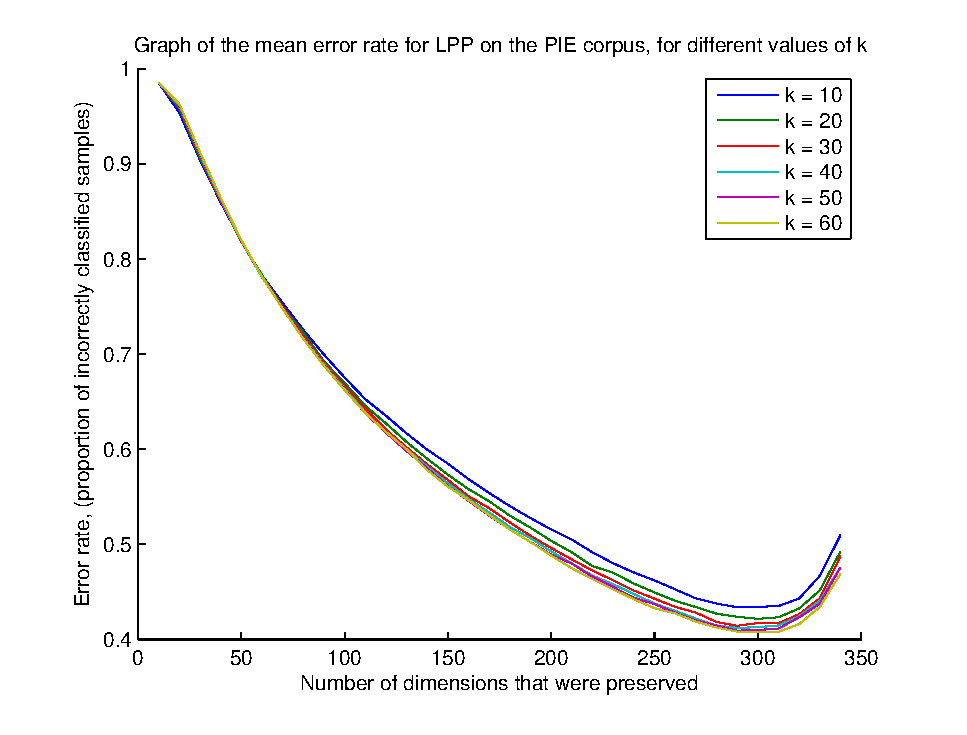
\includegraphics[width=\textwidth]{LPP_vary_k_pie}\label{fig:lpp_pie_graph}}
\subfigure[]{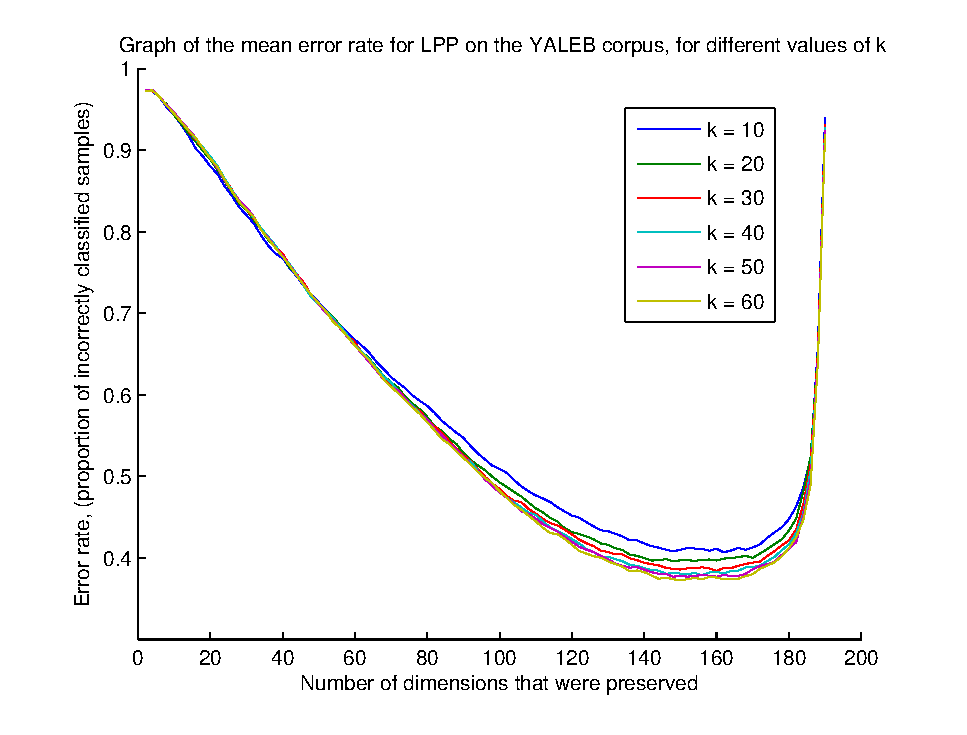
\includegraphics[width=\textwidth]{LPP_vary_k_yaleb}\label{fig:lpp_yaleb_graph}}
\end{figure}

\newpage
\subsection{Fast ICA - Independent Component Analysis}
Fast ICA \cite{ica1} is an algorithm that solves the problem of independent component analysis. Given a set of \(F\) components (e.g. signals, dimensions of training data) on \(N\) training data samples, return a transformation matrix that de-mixes the input into a set of \(F\) independent components. Dimensionality reduction is performed by only mapping the data to the most important components. The returned transformation matrix is of a slightly different form to the matrix returned by the other methods, instead of having dimensionality \(F \times C\) (where \(C\) is the number of reduced dimensions), it has dimensionality \(C \times F\). So it must be transposed before being used on the input data.

\subsubsection{Algorithm}
\begin{enumerate}
\item for \(p\) in the range 1 to \(C\) (\(C\) is the number of desired components):

\begin{enumerate}
\item initialise \(wp\), the vector that will express the pth component, to random numerical values. it has dimensionality \(F \times 1\).
\item for i in the range 1 to num\_iterations:

\begin{enumerate}
\item iteratively update wp, with respect to the observed data and the previously considered wp vectors.
\end{enumerate}

\item store wp as a row in the \(C \times F\) matrix \(X\)

\end{enumerate}

\item return the matrix \(S\) (dimensionality \(C \times F\)), which consists of all of the past wp vectors (one for every p value considered), multiplied by the input data, \(X\)

\end{enumerate}

As Fast ICA is an iterative algorithm that approximates an optimal solution, the more iterations that take place, the better the results will be but the longer the algorithm will take to run. A possible experiment would be to run Fast ICA with different number of iterations, but I did not have time to compute this.


%----------------------------------------------------------------------------------------
%	MAJOR SECTION X - TEMPLATE -  UNCOMMENT AND FILL IN
%----------------------------------------------------------------------------------------


\section{Evaluation}
To compare the performance of all of the different methods, I ran them all on the PIE and YALEB facial recognition problems. Fast ICA was run with the number of iterations set to 10 and LPP was run with a k value of 50. The PIE problem consisted of 340 training data samples and the YALEB problem consisted of 190.

Figure \ref{fig:PIE_error} and \ref{fig:YALEB_error} show the results. The error rate decreases with every method as the number of dimensions is increased, but the error for PCA/whitening starts to increase at 250 on PIE and 150 on YALEB - this could be due to over-specialisation, that is, the model has become unable to generalise to predict unseen data points. The error rate for LPP also curves upwards at 300 for PIE and 160 for YALEB, presumably for the same reason.

From the graphs it is possible to determine that PCA/whitening is the best method overall at any dimensionality, then either LDA or LPP, then PCA, then Fast ICA. I have some comments as to why this result may have occurred:

\begin{itemize}
\item Fast ICA achieved the worst error rate, because the distribution of the data is not appropriate for independent component analysis. ICA exploits the non-Gaussianity of the input data, so it may have performed badly because the data is normally or normally distributed. It also assumes that the original signals are independent. A way to test this hypothesis would be to calculate the non-Gaussianity of the data using a measure such as kurtosis or negentropy.
\item PCA removes covariance, but it does not normalise the variances. This means that if one dimension has a high variance, then it could bias the decision made by the classifier.
\end{itemize}

In the original research paper for LPP \cite{localitypreserve}, it performs better than PCA and LDA on the YALEB facial recognition task, with an error rate of 16\% (or 0.16) which is much lower than the lowest error rate in my experiment (about 0.4, or 40\%). In this paper, PCA has an error rate of 25.3\% and LDA has an error rate of 20\%. Some of the parameters are different (e.g. the images are 32 by 32 pixel grayscale, compared with 64 by 64 in this experiment) but even so, this hints that further improvement may be possible.

\begin{figure}[ph!]
\centering
\subfigure[]{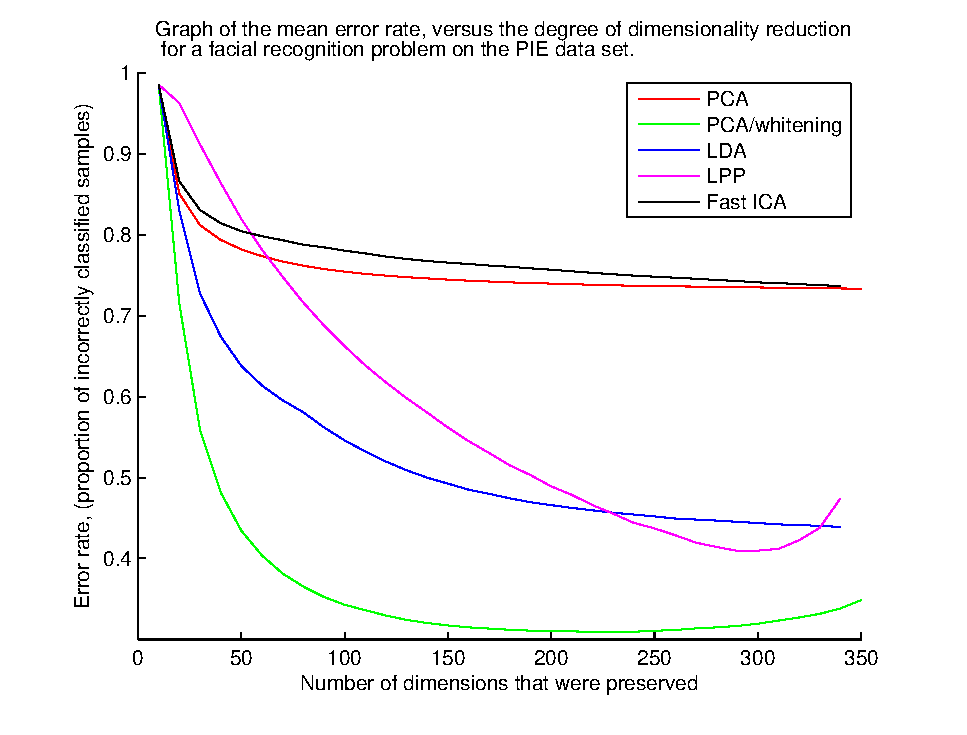
\includegraphics[width=\textwidth]{error_pie}\label{fig:PIE_error}}
\subfigure[]{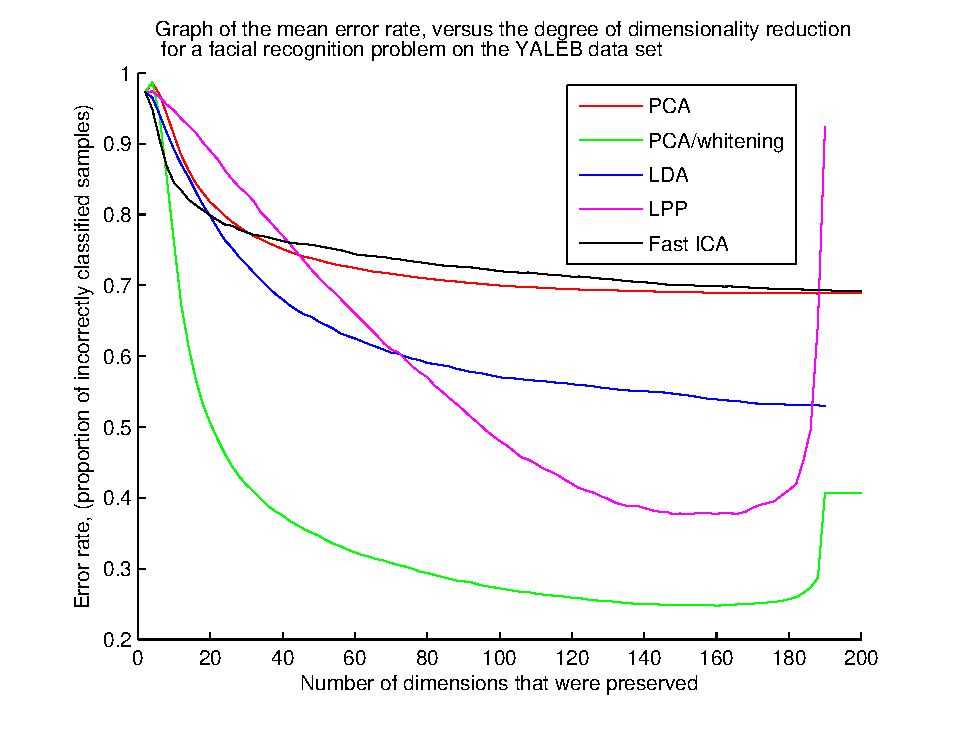
\includegraphics[width=\textwidth]{error_yaleb}\label{fig:YALEB_error}}
\end{figure}


%----------------------------------------------------------------------------------------
%	CONCLUSION
%----------------------------------------------------------------------------------------

\section{Conclusion} % Major section
In this report, I described the PCA, PCA with whitening, LDA, LPP and Fast ICA algorithms as well as presented an evaluation of their performance on the PIE and YALEB facial classification tasks. In the appendix, the Matlab code used to implement them is enclosed, which contains comments about the algorithms. PCA with whitening achieved the lowest error rate, then LPP, LDA, PCA and Fast ICA. If I had more time, I would have investigated the effect of changing the number of iterations made by the Fast ICA algorithm and measured the running times of each algorithm.

%----------------------------------------------------------------------------------------
%	BIBLIOGRAPHY
%----------------------------------------------------------------------------------------

\begin{thebibliography}{99} % Bibliography - this is intentionally simple in this template

\bibitem[Figueredo and Wolf, 2009]{Figueredo:2009dg}
Figueredo, A.~J. and Wolf, P. S.~A. (2009).
\newblock Assortative pairing and life history strategy - a cross-cultural
  study.
\newblock {\em Human Nature}, 20:317--330.
 
\bibitem[Yu L]{dimensionality}
Lei Yu, Jieping Ye and Huan Liu.
\newblock Dimensionality Reduction for Data Mining - Techniques, Applications and Trends (Lecture notes)
\newblock http://www.cs.binghamton.edu/~lyu/SDM07/DR-SDM07.pdf (accessed 22/02/15)

\bibitem[He, Niyogi, 2004]{localitypreserve}
He, X and Niyogi, P.
\newblock Locality Preserving Projections
\newblock http://papers.nips.cc/paper/2359-locality-preserving-projections.pdf

\bibitem[Hyvärinen, A]{ica1}
Hyvärinen, A and Oja, E.
\newblock Independent Component Analysis: Algorithms and Applications
\newblock http://www.cs.helsinki.fi/u/ahyvarin/papers/NN00new.pdf (accessed 22/02/15)

\bibitem[Hyvärinen, A]{ica2}
Hyvärinen, A
\newblock Fast and Robust Fixed-Point Algorithms for Independent Component Analysis
\newblock http://www.cs.helsinki.fi/u/ahyvarin/papers/TNN99new.pdf (accessed 22/02/15)

\bibitem[Hyvärinen, A]{icawiki}
FastICA
\newblock http://en.wikipedia.org/wiki/FastICA (accessed 22/02/15)
\end{thebibliography}

%----------------------------------------------------------------------------------------

\section{Appendix - Code}


\linespread{1} % Line spacing

\lstinputlisting{PCA.m}
\lstinputlisting{PCAWhitening.m}
\lstinputlisting{LDA.m}
\lstinputlisting{LPP.m}
\lstinputlisting{FastICA.m}
\lstinputlisting{KNearestNeighbours.m}



\end{document}